\documentclass[12pt]{article}

\usepackage{hyperref}

% useful for formatting (align*, etc.) and for certain symbols (the QED box, etc.)
\usepackage{amsmath, amssymb, amsthm}

% for including graphics
\usepackage{graphicx}

% for conveniently specifying the spacing (\singlespacing, \doublespacing,
%    \onehalfspacing, etc.)
\usepackage{setspace}
\onehalfspacing

% this does some sort of symbol stuff
\usepackage{textcomp}

% A package for conveniently adjusting headers and such
\usepackage{fancyhdr}
\renewcommand{\headrulewidth}{0 pt}
\rhead{\textit{\thepage}}
\cfoot{}



% Set the margins
\usepackage[top=1.8cm, bottom=1.8cm, left=1.8cm, right=1.8cm]{geometry}

% Differently spaced itemize
\newenvironment{itemize*}%
  {\begin{itemize}%
  	\setlength{\parsep}{0pt}
    \setlength{\itemsep}{0pt}%
    \setlength{\parskip}{0pt}}%
  {\end{itemize}}
\newenvironment{enumerate*}%
  {\begin{enumerate}%
  	\setlength{\parsep}{0pt}
    \setlength{\itemsep}{0pt}%
    \setlength{\parskip}{0pt}}%
  {\end{enumerate}}


% set up a new command to insert a little bit of vertical space
% (use this BEFORE a line break)
\newcommand{\padding}{\vspace*{.5cm}}

% set up an environment to format each hw problem in
\newenvironment{problem}[1]{\noindent\textbf{#1.}}{\vspace*{.5cm}}

\newenvironment{proof*}{\par\noindent{\bf Proof}\quad}
               {\quad\vrule height 8pt depth 0pt width 8pt\medskip\par}



\begin{document}

%Add in some nice looking pages
 \begin{titlepage}
    \vspace*{\fill}
    \begin{center}
      {\Huge Final Report: Android Development Team}\\[0.5cm]
      {\Large Jillian Andersen, Jordan Apele, David Ruhle, Kyle Wenholz}\\[0.4cm]
      \today
    \end{center}
    \vspace*{\fill}
  \end{titlepage}
  
\tableofcontents
\newpage

%Cover Page (include group name and team member names)
%Table of contents

\section{The Final Product}
\label{sec:finalProduct}
%Describe in detail the end product your department is producing, do not 
%    forget about documentation artifacts.

The final product of this development team will be a downloadable Android 
application for playing Pong via human motion.  Receiving position data 
from a Wii Remote the application allows a user to move a paddle on screen 
with motion in physical space.  The current concept is to host games over 
the internet and allow play between two players to proceed as a normal game
 of Pong.  This may change in the future to include \textit{enhanced modes} 
where players may retrieve power-ups, attack or complete any other number 
of non-standard actions.  Aside from the gameplay, however, the Android 
application will host a suite of other features.  Accessing user statistics, 
global statistics, help and support, changing aesthetic settings, adjusting 
the volume, and even navigating to the Vir-Pong website will all be possible 
from within the application.  While the application developed by our team is 
targeted at the Android platform, our team is working closely with the iOS 
development group to support a cohesive and quality application across 
multiple platforms.  

Installation and usage instructions as well as help and support will be 
found on the Android market or on the Vir-Pong site.  These instructions 
will be targeted towards novice technology users so that our product may be
 enjoyed by all groups.  Developer documentation generated during the 
development cycle will be available to all Vir-Pong employees and the 
general public as part of our open-source commitment.  
Where this documentation will be hosted is currently under consideration.  

The final product of this team will integrate with the greater Vir-Pong 
ecosystem.  Servers, devices, the website, and users will bring together a 
community of human Pong players, all enjoying our product.  Our piece in 
this greater puzzle is to put that experience in the pockets of consumers 
and allow Pong to be played in the physical world.

\section{Requirements Analysis}
\label{sec:requirements}

\subsection{Functional Requirements}
\label{sec:functionalRequirements}
%Functional Requirements:
%    Use Cases:
%        All uses cases must use the same template and this template should 
%            identify Actors, Preconditions, Postconditions, Scenario, and 
%            Alternatives for fully-dress uses cases. The template should 
%            also include a meaningful name for the use-case and some form of
%            versioning.
%        Fully Dressed Descriptions: You need to write fully-dressed well 
%            detailed use case for all features you plan to include in your 
%            final product. 

\singlespacing
\subsubsection{Playing a Game - v1.0}
Actors:
\begin{itemize*}
\item Player
\item Hub
\item Android device
\item Input device
\end{itemize*}
Preconditions:
\begin{itemize*}
\item Player is authenticated into the system and has successfully 
  requested a game from the hub.
\item Input device is tethered to the Android device and is ready to 
  submit motion data.
\end{itemize*}
Postconditions:
\begin{itemize*}
\item A winner has been determined.
\item Replay is saved to the system database.
\end{itemize*}
Scenario:
\begin{enumerate*}
\item Hub signals a ready-start and the game begins. 
\item \label{playerObserves}Player observes ball and opponent's paddle 
  motion on Android device.
\item Player responds with appropriate motion, detected by the input 
  device and relayed to the Android device.
\item Android device relays motion data to the hub.
\item \label{HubUpdateGame}Hub recalculates ball and paddle position then 
  sends updated information to Android device.
\item \label{DisplayCurrentInformation}Player's Android device displays 
  the current information.\\
Repeat \ref{playerObserves} through \ref{DisplayCurrentInformation} until 
  a point is scored.
\item \label{LogPointRefresh}Hub logs point scored then resets game state 
  to fresh.\\
Repeat \ref{playerObserves} through \ref{LogPointRefresh} until score limit 
  is reached.
\item \label{AnnounceWinner}Hub indicates winner to Android device.
\item Android device displays winner to player and announces game complete.
\item Hub logs game replay for later access.
\item Player is prompted to play another game or exit back to the home screen.
\end{enumerate*}
Alternatives:\\
\ref{HubUpdateGame}a) Hub signals that connection to other player has 
  been lost.
\begin{enumerate*}
\item Android device pauses the game and signals a disconnection from the game.
\item Player is prompted to leave the game.
\item The player goes back to main menu.
\end{enumerate*}

\begin{figure}
\begin{center}
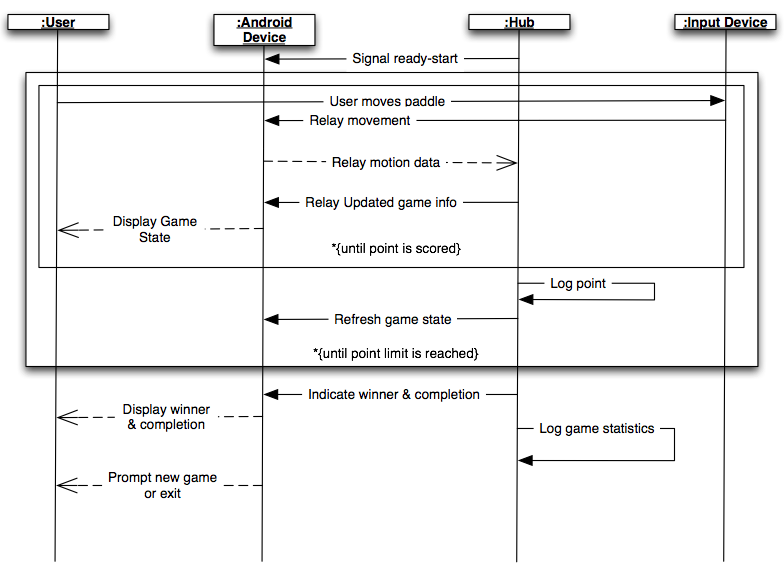
\includegraphics[scale=.5]{ssd_GamePlay_1.png}
\caption{\label{ssd_GamePlay_1}The role of our system in gameplay is 
  described through the system sequence diagram above.}
\end{center}
\end{figure}


\subsubsection*{Initializing a Game - v3.0}
Actors:
\begin{itemize*}
\item Player
\item Hub
\item Device
\end{itemize*}
Preconditions:
\begin{itemize*}
\item The application is installed and open on the device.
\item The player has already created an account with Vir-Pong.
\item The input device is tethered to the Android device and is ready to 
  submit motion data.
\end{itemize*}
Postconditions:
\begin{itemize*}
\item The hub is relaying game information.
\item The system is using a display to relay the game state.
\end{itemize*}
Scenario:
\begin{enumerate*}
\item \label{InitGame_DisplayOptions} The software displays various options.
\item \label{SelectStart}The player selects to begin a game.
\item \label{DisplayGameRooms} The player is prompted with a list of various
game rooms.
\item \label{SelectRoom} Player selects the desired game.
\item \label{SystemRequestsGame}The device requests the selected game from 
the hub.
\item \label{NotifyPaddle} The player is notified of which paddle she is.
\item \label{HubSelectsOpponent}The hub waits for an opponent then signals a 
  ready-start to device.
\item \label{LoadGameState}The device loads an initial game state displayed 
  to the player.
\item Game begins.
\end{enumerate*}
Alternatives:\\
\ref{SelectStart}a) The player selects the wrong action.
\begin{enumerate*}
\item The player may elect to go back the the previous screen with a 
  $return$ function.
\end{enumerate*}

\ref{SystemRequestsGame}a) The system can not connect to the hub.
\begin{enumerate*}
\item The device sends the player an error message that prompts the player 
  to retry or exit.
\item Player chooses to retry.
\item System connects to hub.
\item Return to \ref{HubSelectsOpponent} of main scenario.
\end{enumerate*}

\subsubsection*{Connect to Input Device - v2.0}
Actors:
\begin{itemize*}
\item Player
\item Device 
\item Wii Remote
\end{itemize*}
Preconditions:
\begin{itemize*}
\item System is installed on the device and has launched.
\end{itemize*}
Postconditions:
\begin{itemize*}
\item Input device (Wii Remote) is selected and prepared for game use.
\end{itemize*}
Scenario:
\begin{enumerate*}
\item Player is prompted with options for input devices.
\item \label{SelectInput} Player selects to use a Wii Remote, but Wii Remote
is not connected yet.
\item \label{PromptToConnect} Device directs player to instructions for 
pairing with a Wii Remote.
\item \label{MenuToWii}Following directions, the player opens the correct 
menu for pairing with a Wii Remote.
\item Player selects to pair with the Wii Remote.
\item \label{ConnectWiimote}System attempts to tether Wii Remote.
\item Player follows instructions from system to connect Wii Remote.
\item System accepts Wii Remote device and notifies user.
\end{enumerate*}
Alternatives:\\
\ref{SelectInput}a) Player selects phone accelerometer.  
\begin{enumerate*}
\item System asks player to make certain the device has an built in 
  accelerometer.
\item Player indicates that device has accelerometer.
\item System connects to device accelerometer.
\item System proceeds to game launch.
\end{enumerate*}
\ref{SelectInput}b) Player selects touch screen interface.
\begin{enumerate*}
\item System asks player to touch a box displayed on-screen to ensure 
  that a touch screen is available.
\item Player touches box.
\item System proceeds to game launch.
\end{enumerate*}
\ref{ConnectWiimote}System attempts Wii Remote connection, and fails.
\begin{enumerate*}
\item System alerts user that connection failed.
\item User is prompted to try again or back out.
\end{enumerate*}

\subsubsection*{Changing the Game Settings - v2.0}
Actors:
\begin{itemize*}
\item Player
\item Device
\end{itemize*}
Preconditions:
\begin{itemize*}
\item The application is installed and open on the device.
\end{itemize*}
Postconditions:
\begin{itemize*}
\item The newly changed settings have been saved and will be applied to 
  future game play.
\end{itemize*}
Scenario:
\begin{enumerate*}
\item Main menu options are displayed to the player.
\item \label{SelectChangeSettings}Player selects a $change$ $settings$ 
  function.
\item \label{ChangeSettings}Player changes the setting(s).
\item \label{SelectSave}Player selects a $save$ $and$ $apply$ function.
\item \label{SystemSaves}Device saves changes and applies them to future 
  game plays.
\item \label{ReturnToMainMenu}Device returns to the main menu.
\end{enumerate*}
Alternatives:\\
\ref{ChangeSettings}a) The player selects a non-valid entry for a setting.
\begin{enumerate*}
\item The device displays an error message that tells the player he 
  entered a non-compatible value.
\item The device returns the setting to a default state.
\end{enumerate*}
\ref{SelectSave}a) The player decides not to change any settings.
\begin{enumerate*}
\item The player selects the $return$ function.
\end{enumerate*}
\onehalfspacing

\singlespacing
\subsubsection*{Viewing Replays - v2.0}
Actors:
\begin{itemize*}
\item Player
\item Website
\item Device
\end{itemize*}
Preconditions:
\begin{itemize*}
\item Our application is installed on the device and has launched.
\item The player has already created an account with Vir-Pong and is logged
  in.
\end{itemize*}
Postconditions:
\begin{itemize*}
\item The player has watched their replay.
\end{itemize*}
Scenario:
\begin{enumerate*}
\item Main menu options are displayed to the player.
\item \label{SelectReplay}Player chooses to view replay.
\item \label{ReplayChoice}Device requests list of available replays from server.
\item Database sends list of replays.
\item Device displays list of replays.
\item \label{WatchReplay}Player selects a replay to watch.
\item Device displays replay.
\item \label{Back}Player finishes the replay and hits the back button.
\item Device returns to main menu.
\end{enumerate*}
Alternatives:\\
\ref{PersonalStatRequest}a) Unable to obtain available replays.
\begin{enumerate*}
\item Display connection error message.
\item Player may utilize a $retry$ or $continue$ button.
\item Player selects $retry$.
\item Return to \ref{PersonalStatRequest}.
\end{enumerate*}

\subsubsection*{Editing Account Information - v1.0}
Actors:
\begin{itemize*}
\item Player
\item System
\item Vir-Pong Website
\end{itemize*}
Preconditions:
\begin{itemize*}
\item The application is installed on the device and has launched.
\end{itemize*}
Postconditions:
\begin{itemize*}
\item Player has edited account information.
\end{itemize*}
Scenario:
\begin{enumerate*}
\item Player selects Edit Account information on main menu.
\item Device displays current login and pin number.
\item Player may change these current settings.
\item Player saves and exits editing account information.
\item System returns user to previous page.
\end{enumerate*} 

\onehalfspacing



%    System Sequence Diagram:
%        Create a system sequence diagram for your most important 
%        fully-dressed use case. Include a one paragraph description of what 
%        is being depicted in the diagram (use plan English). 



\subsection{Nonfunctional Requirements}
\label{sec:nonfunctionalRequirements}
%Nonfunctional Requirements: Detail all nonfunctional requirements that you 
%    addressed in your final product (e.g. Easy Visibility: All text in our 
%    product is 16pt font.)


\subsubsection{Usability Requirements}
%Human factors, Aesthetics, Consistency, Documentation
In order for the application to provide an experience enjoyable to a wide 
user base, the following usability requirements should be met:
\begin{itemize}
\item Players should have their statistics saved and then made available 
for viewing.
\item Players should be able to change game settings(difficulty, ball shape, 
etc.).
\item Users should be able to register an account through the application.
\item The application needs to be available for download via the website 
or on the Android Market.
\item The application should have the option to view a game in progress.
\item It would be nice to make the game environment modifiable (i.e. theming).
\item When there is not a second available human player (or connection to 
the hub is impossible) there should be an option for playing versus the 
computer in training mode.
\end{itemize}

\subsubsection{Reliability Requirements}
%Frequency/severity of failure, Recoverability, Predictability, Accuracy, 
%Mean time to failure
A working product is important, but reliability ensures a consistent 
experience.  With this in mind, our design is striving for security of 
private user information and the ability to pause the game.  The latter is 
focused on creating a fault tolerant solution for network connectivity.  A 
strict testing policy will help to alleviate many other possible issues.

\subsubsection{Performance Requirements}
%Speed, Efficiency, Resource consumption, Throughput, Response time
The ability to adjust the display for different screens will allow for 
better performance of the software on different Android devices.  The system 
must also minimize latency when contacting the server for game information 
or receiving information from the Wii Remote.  There are no other connections 
that are quite as important.

\subsubsection{Supportability Requirements}
%Testability, Extensibility, Adaptability, Maintainability, Compatibility, 
%Configurability, Serviceability, %Installability, Localizability, Portability
Installation, game play, and resource usage should all be properly 
documented in a conveniently located and navigated user-manual. A list of 
known compatible devices included in the manual will assist in keeping 
potential customers informed about our product.  There should also be some 
contact information for support and help when the available documentation 
is not enough.

In keeping with the project's open source roots, it will be important to 
make all source code well documented for the general public; make the 
source code readily available; give credit to non-employees that have 
contributed to our application; and provide substantial developer 
documentation. 




\section{Diagrammatic Depictions of the Product}
\label{sec:diagrams}
%Domain Analysis: Create a UML diagram that depicts the domain model for your
%    product (this will be a revision from Report 1). Include a plain-English
%    description of what is being shown in the diagram. Define any terms used
%    in conceptual classes, attributes, or associations that might not be 
%    clear to a lay person.


%Interaction Diagram:
%    Create an interaction diagram for each of the events depicted in your 
%    System Sequence Diagram.
%    Add a description of the design principles (Information Expert, Creator,
%    High Cohesion, Low Coupling, Controller) you employed, where you employed
%    them and why you made those choices. 

\section{Implementation}
\label{sec:implementation}
%Implementation:
%    Include the coding style guide that your team is using. This should be 
%    fairly detailed including naming, coding conventions, and comment 
%    conventions.
%    Install documentation: include a description of all necessary procedures 
%    a developer would have to complete to install your product. If you are 
%    assuming a certain starting environment then explicitly state so (e.g. a 
%    Linux server with Apache installed). Make sure to include how the user 
%    would access and download your source code and documentation. If you had 
%    difficulty installing from the previous teams description be sure to 
%    correct those difficulties.
%    Include a current class diagram of your product
%        Diagram should depict all classes and their associations 
%    Description of algorithms, data structures and design patterns
%        Describe any complex algorithms, data structures, or design patterns 
%        your group used. Provide insights as to why you made the choices you 
%        did.
%        Describe any techniques you are using to ensure fault tolerance (e.g.
%        if you have information to write to a db but the db is down what do 
%        you do?) 
%    Data Storage:
%        Identify all the data you are storing (ex. user athentication, 
%        medical records, back up information if the DB is down etc.)
%        If your product contains a database include both an ER Diagram and 
%        the schema for it, include a description of why you made the design 
%        decisions you did.
%        If the data is not stored in a db describe how it is stored included 
%        formatting. 
%    Describe your testing and verification procedure for your implemented 
%    code 

\section{Developer Documentation}

\label{sec:developerdocumentation}

\subsection{Setting up the Development Environment}
In order to develop for Android, you will need the Android SDK, the PhoneGap software, and some editor (for example, Eclipse).  These pieces are relatively easy to set up, but because all systems are different, some personal configuration may be required.  All of the software mentioned below can be found, with current links, at the PhoneGap Android page\cite{PhoneGap-Android}.  

\subsubsection{Android SDK}
The Android SDK comes with an Android Emulator as well as Android libraries.
To download the SDK, first check to make sure your operating system fulfills all of the system requirements.  A list of of system requirements is available on the Android Developers website\cite{AndroidSDK-SystemRequirements}.

Next, download the Android SDK from the Android Developer website\cite{AndroidSDK-Download}.
The instructions for installation are found on the same site but on the installation page\cite{AndroidSDK-Installation}. \textbf{Note:} do not put a space in the folder name.

After that, you must add necessary components to the SDK.  The instructions for that portion are found on the components page\cite{AndroidSDK-Components}.  On your first run, you will be required to create an Android Virtual Device (AVD) that is simply a mock phone.


\subsubsection{PhoneGap}
The PhoneGap download is primarily a collection of tools that provide functionality for the HTML5 and JavaScript interface in a native application environment.  That is, the PhoneGap jar, js, and xml files all serve to support the use of HTML5 and JavaScript coding as implementing the core functionality of the application.  The download for PhoneGap can be found on the PhoneGap Android page\cite{PhoneGap-Android}.


\subsubsection{Editing Environment}
In theory, any development can be done from a text editor so long as you have access to the Android SDK and Java.  It is highly recommended, however, that you use Eclipse\cite{Eclipse-Helios}.  You then may want to install the ADT plugin for Android Development\cite{Eclipse-ADT}.  In addition, you may then want to install the plugin for PhoneGap Development\cite{PhoneGap-Eclipse}.

\textbf{An important note:} When creating a PhoneGap application in Eclipse, it may be necessary to include the PhoneGap jar file in the libs folder of the application.  To do this, right-click on the Eclipse project, and select "Build Path", then "Configure Build Path".  If there is no PhoneGap jar file included, then select to "Add External JARs".  Select the jar file downloaded earlier with the rest of the PhoneGap tools and click "Okay".

\subsection{Retrieving the Source}
<<<<<<< HEAD
In order to work with the source code of the project, you will likely want to use Git\cite{Github}.  Using Git, you may clone the repository from \url{git@github.com:VirPong/human-pong}.  You will then want to navigate into $Android/VirPong-Mobile/$ and create a folder called $assets$.  Navigate into $assets$ and clone \url{git@github.com:VirPong/www}.  Now you may open Eclipse and import the $VirPong-Mobile$ directory as an existing project.  You may need to point the build path to your PhoneGap Jar file (located wherever you downloaded PhoneGap and then inside the Android folder).  Once this is done, you may begin development!  \textbf{Note:} an alternative to git is to download the repository from \url{https://github.com/VirPong/human-pong} and \url{https://github.com/VirPong/www}, placing the $www$ repository in the same place mentioned above.
=======
In order to work with the source code of the project, you will likely want to use Git\cite{Github}.  Using Git, you may clone the repository from \url{git@github.com:Vir-Pong/human-pong}.  You will then want to navigate into $Android/Vir-Pong-Mobile/$ and create a folder called $assets$.  Navigate into $assets$ and clone \url{git@github.com:Vir-Pong/www}.  Now you may open Eclipse and import the $Vir-Pong-Mobile$ directory as an existing project.  You may need to point the build path to your PhoneGap Jar file (located wherever you downloaded PhoneGap and then inside the Android folder).  Once this is done, you may begin development!  \textbf{Note:} an alternative to git is to download the repository from \url{https://github.com/Vir-Pong/human-pong} and \url{https://github.com/Vir-Pong/www}, placing the $www$ repository in the same place mentioned above.
>>>>>>> upstream/master

\section{Reflections}
\label{sec:reflections}
%Reflections:
%    Describe the technical challenges you encountered in the development of 
%    your product.
%    Describe how the software engineering techniques you learned in this 
%    course helped you in your development.
%    Describe what you would have done differently if you were to start this 
%    project over again.
%    If you were to continue this project what would you do. 



%%%%%%%%%%%%%%%%%%%%%%%%%%%%%%%%%%%%%%%%%%%%%%%%%%%%%%%%%%%%%%%
%8. References: Clearly indicate all the tools and sources you have used in the development of your product thus far. 
%%%%%%%%%%%%%%%%%%%%%%%%%%%%%%%%%%%%%%%%%%%%%%%%%%%%%%%%%%%%%%%


\newpage
\bibliographystyle{amsplain}
\bibliography{finalReport.android.bib}








\end{document}